% Origami Verse whitepaper, version 1.0 (November 2026).
% Build: pdflatex origami-verse-whitepaper.tex (twice). No bibtex step: the references are inline.
\documentclass[11pt,a4paper]{article}

\usepackage[T1]{fontenc}
\usepackage[utf8]{inputenc}
\usepackage{lmodern}
\usepackage{microtype}
\usepackage[margin=2.5cm]{geometry}
\usepackage{amsmath,amssymb}
\usepackage{booktabs}
\usepackage{tabularx}
\usepackage{array}
\usepackage[dvipsnames]{xcolor}
\usepackage{enumitem}
\usepackage{titlesec}
\usepackage{caption}
\usepackage{float}
\usepackage{fancyhdr}
\usepackage{tikz}
\usetikzlibrary{arrows.meta,positioning,calc,fit,shapes.geometric,decorations.pathreplacing}
\usepackage[colorlinks=true,linkcolor=NavyBlue,citecolor=NavyBlue,urlcolor=NavyBlue]{hyperref}
\hypersetup{pdftitle={Origami Verse: Conditional Markets and Worst-World Lending on NEAR},pdfauthor={The Origami Verse team}}

\definecolor{ifv}{HTML}{3B4BA8}
\definecolor{ifvlight}{HTML}{E8EBF8}
\definecolor{good}{HTML}{2E7D32}
\definecolor{bad}{HTML}{C62828}
\definecolor{note}{HTML}{F5F5F0}

\titleformat{\section}{\large\bfseries\color{ifv}}{\thesection}{0.8em}{}
\titleformat{\subsection}{\normalsize\bfseries}{\thesubsection}{0.8em}{}
\setlist{itemsep=2pt,topsep=4pt}
\captionsetup{font=small,labelfont=bf}
\setlength{\parskip}{3pt}

\pagestyle{fancy}
\fancyhf{}
\fancyhead[L]{\small Origami Verse whitepaper v1.0}
\fancyhead[R]{\small November 2026}
\fancyfoot[C]{\small\thepage}
\renewcommand{\headrulewidth}{0.3pt}

% World names of the running example (two events: SPICE, then the December Fed meeting).
\newcommand{\wSC}{\textsf{SHIPS$\cdot$CUTS}}
\newcommand{\wDC}{\textsf{DELAYED$\cdot$CUTS}}
\newcommand{\wSH}{\textsf{SHIPS$\cdot$HOLDS}}
\newcommand{\wDH}{\textsf{DELAYED$\cdot$HOLDS}}
\newcommand{\code}[1]{\texttt{\small #1}}
\newcommand{\tx}[2]{\href{https://testnet.nearblocks.io/txns/#1}{\code{#2\ldots}}}
\newcommand{\inwords}[1]{\par\noindent\colorbox{note}{\parbox{\dimexpr\linewidth-2\fboxsep}{\small\textit{In plain words.} #1}}\par}

\title{\vspace{-1.5em}\textbf{Origami Verse: Conditional Markets and Worst-World Lending on NEAR}\\[0.4em]
\large Version 1.0}
\author{The Origami Verse team\\[0.3em]
\small \url{https://multiverse-lending.vercel.app}\\
\small \url{https://github.com/skyyycodes/multiverse-near}}
\date{November 2026}

\begin{document}
\maketitle
\thispagestyle{fancy}

\begin{abstract}
\noindent
Origami Verse is a protocol on NEAR that lets people hold, trade and borrow against an asset \emph{one possible future at
a time}. A market is built from one to three real-world yes/no events. Every combination of their outcomes is a
\emph{world}, so a market has two, four or eight worlds. One real token can be split into one conditional token per
world; each conditional token pays out only if its world is the one that comes true. Each world has its own pool
and order book, so a holder can keep NEAR in the futures they like and swap it for dollars in the futures they fear.
Lending values a borrower's position in every world that is still possible and sizes the loan by the
\emph{worst} of them, so the collateral covers the debt whichever world happens. The protocol adds three lending
tiers (Safe, Normal, Bold), liquidation that pays in tokens or in cash, an insurance reserve, markets that anyone
can propose and fund with pledges, resolution from public sources with a dispute window and an optional run inside
a trusted execution environment, and an outside NEAR/USD check taken from four public price sources. Everything runs in one
Rust contract on NEAR testnet. This paper explains the model, the maths and the implementation in plain words, with
the real parameters read from the contract and real transactions from the testnet deployment.
\end{abstract}

\setcounter{tocdepth}{1}
\tableofcontents
\vspace{0.5em}

%=====================================================================
\section{Introduction}
\label{sec:intro}

\subsection{The problem}

Suppose you hold NEAR and you have a specific worry: ``If the next big upgrade slips \emph{and} the US central bank
does not cut rates, NEAR will fall.'' Today you have two blunt tools. You can sell NEAR, or you can buy a put option.
Both protect you in \emph{every} future, including the futures you expect to go well, and you pay for that
protection everywhere. A prediction market lets you bet on one event, but it does not let you say ``keep my NEAR if
the upgrade ships, turn it into dollars if it does not''. A lending market does not accept such a position as
collateral at all.

Origami Verse fixes this by cutting an asset along the lines of possible futures. You protect yourself only in the futures
you fear, you keep your upside in the others, and you can still borrow real dollars against the result.

\subsection{The idea in one picture}

Take two real events:
\begin{itemize}
  \item Event 1: ``Will SPICE ship on NEAR mainnet by Mar 31, 2027?'' Outcomes: \textsf{SHIPS} or \textsf{DELAYED}.
  \item Event 2: ``Will the Fed cut at its December 8--9, 2026 meeting?'' Outcomes: \textsf{CUTS} or \textsf{HOLDS}.
\end{itemize}
Together they describe four possible futures, which we call \emph{worlds}: \wSC, \wDC, \wSH{} and \wDH.
Exactly one of them will come true. One wNEAR (wrapped NEAR, a normal token) can be split into four pieces:
``wNEAR if \wSC'', ``wNEAR if \wDC'', and so on. Each piece pays one real wNEAR if its world comes true and
nothing otherwise. Holding all four is the same as holding one wNEAR, because exactly one of them will pay.

The idea of splitting an asset into one version per possible outcome and moving value between those versions comes
from Paradigm's essay ``Multiverse Finance'' \cite{white2025}. Origami Verse is our own design and implementation of
that idea on NEAR, with trading, lending, market creation and resolution built around it.

\subsection{What this paper covers}

Section~\ref{sec:model} defines events, worlds, masks and conditional tokens, and the rules that keep every token
fully backed. Section~\ref{sec:trading} explains the pools, the odds and the order book. Section~\ref{sec:prices}
shows how lending reads prices safely. Section~\ref{sec:lending} covers worst-world lending, tiers, interest,
liquidation and bad debt. Section~\ref{sec:catalog} explains how anyone can propose and fund a new market.
Section~\ref{sec:resolution} covers resolution, and Section~\ref{sec:reference} the outside NEAR/USD check.
Section~\ref{sec:near} describes the NEAR implementation, Section~\ref{sec:security} security and invariants,
Section~\ref{sec:eval} the live testnet deployment, and Section~\ref{sec:limits} what is still missing.

\paragraph{Where the numbers come from.} Every parameter in this paper was read from the contract source
(\code{contracts/multiverse/src} and \code{crates/multiverse-math/src}) or from the live contract
\code{app.ifverse-staging.testnet}\footnote{The testnet accounts (\code{*.ifverse-staging.testnet}), the rule tags and the web address keep earlier working names; the project was formerly IfVerse / Multiverse Lending.} on NEAR testnet on 14 November 2026. Prices and balances from the live markets are
snapshots: they move as people trade.

%=====================================================================
\section{The model: events, worlds and verse tokens}
\label{sec:model}

\subsection{Events and outcomes}

An \textbf{event} is a yes/no question about the real world with two named outcomes, a written \textbf{rule} that
says exactly how it resolves, and a public \textbf{source}. For example, event 2 on the live contract has the rule:
``CUTS if both limits of the federal funds target range (FRED DFEDTARU and DFEDTARL) on 2026-12-10 are lower than on
2026-12-08; HOLDS if neither is lower (a hike resolves HOLDS).'' Each rule ends with a short machine tag such as
\code{[ifverse:fomc:2026-12-08:2026-12-10]}, which tells the off-chain tools what data to read. Rules are stored on
chain (up to 1,024 bytes).

\subsection{Worlds and masks}

A \textbf{market} (called a \emph{scenario} in the code) combines $n$ events, with $1 \le n \le 3$. A
\textbf{world} is one combination of outcomes, so a market has $W = 2^n$ worlds: 2, 4 or 8. Worlds are numbered
$0,\dots,W-1$. In world $w$, event $k$ has outcome
\begin{equation}
  o_k(w) = \left\lfloor w / 2^k \right\rfloor \bmod 2 ,
  \label{eq:outcome}
\end{equation}
where outcome 0 is the first named outcome (\textsf{SHIPS}, \textsf{CUTS}, \textsf{YES}) and outcome 1 the second.
\inwords{Write the world number in binary. Bit 0 is the answer to the first event, bit 1 the answer to the second
event, bit 2 the answer to the third. World 2 is binary \code{10}: the first event took outcome 0 (\textsf{SHIPS}),
the second took outcome 1 (\textsf{HOLDS}), so world 2 is \wSH.}

A \textbf{mask} is a set of worlds, written as a number whose bit $w$ is set when world $w$ is in the set. In the
four-world market, mask 1 (\code{0001}) is \wSC{} alone, mask 3 (\code{0011}) is ``the Fed cuts'' (worlds 0 and 1),
mask 5 (\code{0101}) is ``SPICE ships'' (worlds 0 and 2), and mask 14 (\code{1110}) is every world except \wSC.
The mask with every bit set is the \textbf{root}: it means ``in every world'', which is just the real asset.
A four-world market has 15 non-empty masks and an eight-world market 255.

Each market also keeps a mask called \code{possible}: the worlds that can still happen. It starts as the root and
loses worlds as events resolve.

\subsection{Verse tokens}

A \textbf{verse token} is one asset on one mask of one market. ``wNEAR-if-mask-14 in market 1'' pays one real wNEAR
if the world that comes true is in mask 14. Origami Verse supports two assets, wNEAR and USDC, so in every market each
non-root mask has a wNEAR verse and a USDC verse. Each verse is a NEP-245 multi-token \cite{nep245} with the id
\code{\{market\}:\{asset\}:\{mask\}}, for example \code{1:wnear:14}.

A verse is \emph{live} while its mask still contains a possible world, \emph{dead} once it does not, and
\emph{collapsed} once its mask contains every possible world. A collapsed verse is as good as the real asset: it
redeems one for one.

\subsection{Split, merge and redeem}

Three operations move value between masks. None of them uses a price.

\begin{itemize}
\item \textbf{Split} turns an amount on one mask into the same amount on each part of a partition of that mask. The
parts must not overlap and together must cover every possible world of the parent. Splitting from the root takes
real tokens in and puts them in the market's \textbf{reserves}.
\item \textbf{Merge} is the reverse: equal amounts of all the parts become the parent. Merging into the root pays
real tokens out of the reserves.
\item \textbf{Redeem} pays one real token for each collapsed verse token after resolution.
\end{itemize}

\begin{figure}[t]
\centering
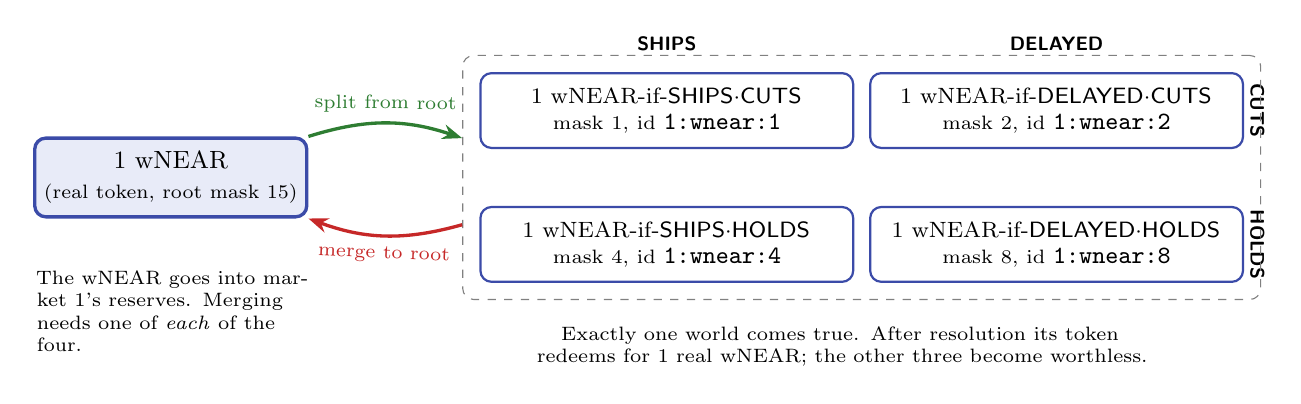
\begin{tikzpicture}[
  font=\small,
  real/.style={draw=ifv,fill=ifvlight,very thick,rounded corners,minimum width=2.6cm,minimum height=1cm,align=center},
  verse/.style={draw=ifv,fill=white,thick,rounded corners,text width=4.5cm,minimum height=0.95cm,align=center,font=\footnotesize},
  >={Stealth[length=2.5mm]}]
  \node[real] (root) at (0,0.6) {1 wNEAR\\\scriptsize(real token, root mask 15)};
  \node[verse] (w0) at (6.3, 1.45) {1 wNEAR-if-\wSC\\\scriptsize mask 1, id \code{1:wnear:1}};
  \node[verse] (w1) at (11.25,1.45) {1 wNEAR-if-\wDC\\\scriptsize mask 2, id \code{1:wnear:2}};
  \node[verse] (w2) at (6.3,-0.25) {1 wNEAR-if-\wSH\\\scriptsize mask 4, id \code{1:wnear:4}};
  \node[verse] (w3) at (11.25,-0.25) {1 wNEAR-if-\wDH\\\scriptsize mask 8, id \code{1:wnear:8}};
  \node[font=\scriptsize\bfseries] at (6.3,2.3) {\textsf{SHIPS}};
  \node[font=\scriptsize\bfseries] at (11.25,2.3) {\textsf{DELAYED}};
  \node[font=\scriptsize\bfseries,rotate=-90] at (13.8,1.45) {\textsf{CUTS}};
  \node[font=\scriptsize\bfseries,rotate=-90] at (13.8,-0.25) {\textsf{HOLDS}};
  \node[draw=gray,dashed,rounded corners,fit=(w0)(w1)(w2)(w3),inner sep=6pt] (grid) {};
  \draw[->,very thick,good] (root.north east) to[bend left=18] node[above,sloped,font=\scriptsize]{split from root} ($(grid.west)+(0,0.5)$);
  \draw[->,very thick,bad] ($(grid.west)+(0,-0.6)$) to[bend left=18] node[below,sloped,font=\scriptsize]{merge to root} (root.south east);
  \node[align=left,font=\scriptsize,text width=3.4cm] at (0,-1.1) {The wNEAR goes into market 1's reserves. Merging needs one of \emph{each} of the four.};
  \node[align=center,font=\scriptsize,text width=8.4cm] at (8.5,-1.55) {Exactly one world comes true. After resolution its token\\redeems for 1 real wNEAR; the other three become worthless.};
\end{tikzpicture}
\caption{Splitting one wNEAR in a market of two events (four worlds). Columns are the outcomes of event 1 (SPICE),
rows the outcomes of event 2 (the December Fed meeting). Splitting and merging never change the total backing.}
\label{fig:split}
\end{figure}

Split and merge only burn and mint, one for one, with no rounding. Reserves move only on a split from the root, a
merge into the root and a redeem. This gives the central rule of the system, the \textbf{backing invariant}: for
every market, every asset and every possible world $w$,
\begin{equation}
  \sum_{\text{masks } M \ni w} \operatorname{supply}(M) \;=\; \operatorname{reserves}.
  \label{eq:backing}
\end{equation}
\inwords{Pick any world that could still happen. Add up every token that would pay out if that world came true.
The total always equals the real tokens locked in the market. So whichever world wins, there is exactly enough real
money to pay everyone who holds a winning token. No price, pool or loan can break this, because they only move
existing tokens between people.}

%=====================================================================
\section{Trading}
\label{sec:trading}

Splitting by itself only changes the shape of what you hold. To \emph{hedge}, you need to swap: give up NEAR in the
worlds you fear and get dollars there instead. Origami Verse offers three kinds of pool and an order book. Internally every
amount is an 18-decimal integer; prices are USDC per wNEAR; fees are counted in \emph{pips}
(1,000,000 pips $=$ 100\%).

\subsection{World pools: the price of NEAR in one world}

A \textbf{world pool} trades wNEAR-if-$w$ against USDC-if-$w$ for a single world $w$. Both sides pay only in world
$w$, so the pool's price is ``what NEAR is worth if world $w$ happens''. Pools are constant-product pools with the
behaviour of a full-range concentrated-liquidity position \cite{uniswapv3}:
\begin{equation}
  x \cdot y = L^2, \qquad p_w = \frac{y}{x},
  \label{eq:cpmm}
\end{equation}
where $x$ is the wNEAR-if-$w$ in the pool, $y$ the USDC-if-$w$, $L$ the pool's liquidity and $p_w$ its price.
\inwords{The pool keeps the product of its two balances fixed. When you sell NEAR into it, $x$ goes up, so $y$ must go
down: you get USDC out, and the price of NEAR in that world falls a little. A bigger pool (larger $L$) moves less for
the same trade.}

On 14 November 2026 the four world pools of market 1 priced NEAR at 4.18 (\wSC), 3.12 (\wDC), 3.44 (\wSH) and
2.66 (\wDH) USDC. The market believes NEAR is worth most if SPICE ships and the Fed cuts, and least if SPICE slips
and the Fed holds.

\subsection{Odds pools: how likely each world is}

An \textbf{odds pool} trades USDC-if-$X$ against USDC-if-$Y$ for two disjoint masks $X$ and $Y$. Because one dollar
in $X$ and one dollar in $Y$ only differ in \emph{when} they pay, their exchange rate is the market's view of how
likely $X$ is compared with $Y$. A pool with reserves $r_X$ and $r_Y$ gives $X$ the share
\begin{equation}
  s_X = \frac{r_Y}{r_X + r_Y}
  \label{eq:share}
\end{equation}
of their common parent. Odds pools form a tree from the root down to single worlds
(Figure~\ref{fig:pools}). A world's probability $q_w$ is the product of the shares along its branch. The second
child of each split takes ``parent minus first child'', so the probabilities always add up to exactly 1. If a split
between two live masks has no pool, the odds are reported as unknown rather than guessed.
\inwords{If USDC-if-CUTS is plentiful in its pool and USDC-if-HOLDS is scarce, ``a dollar if the Fed cuts'' is
cheap and ``a dollar if the Fed holds'' is dear: traders think a cut is unlikely. The pool's balances turn that view
into a percentage.}

\begin{figure}[t]
\centering
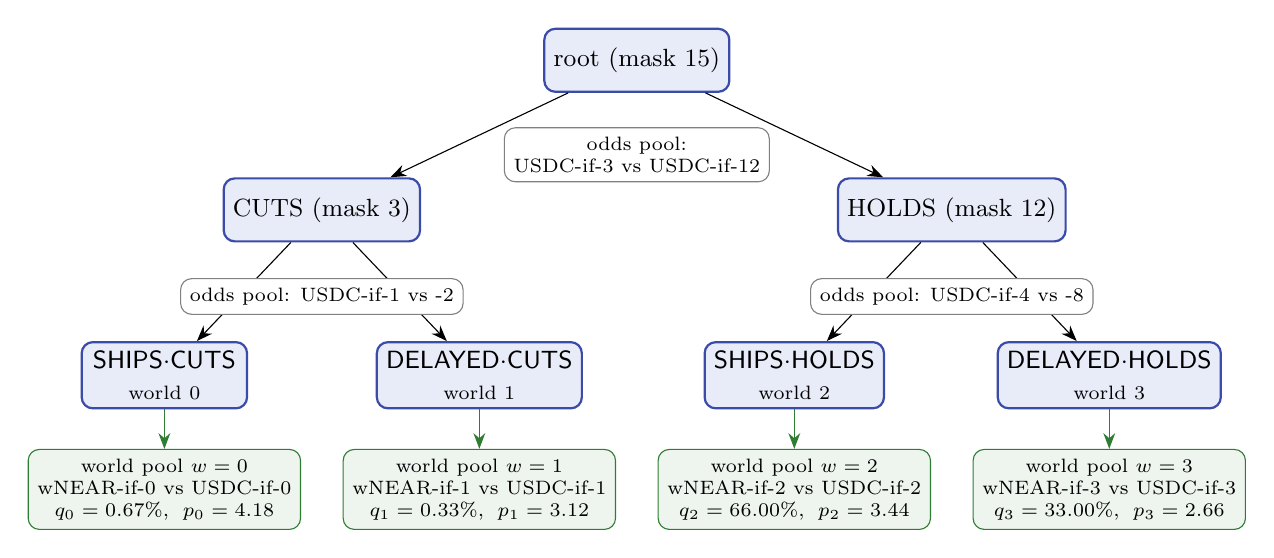
\begin{tikzpicture}[
  font=\small,
  mask/.style={draw=ifv,thick,rounded corners,fill=ifvlight,minimum width=2.1cm,minimum height=0.8cm,align=center},
  pool/.style={draw=gray,fill=white,rounded corners,font=\scriptsize,align=center,minimum width=2.4cm},
  wpool/.style={draw=good,fill=good!8,rounded corners,font=\scriptsize,align=center,minimum width=2.6cm},
  >={Stealth[length=2mm]}]
  \node[mask] (r) at (0,0) {root (mask 15)};
  \node[mask] (c) at (-4,-1.9) {CUTS (mask 3)};
  \node[mask] (h) at (4,-1.9) {HOLDS (mask 12)};
  \node[pool] at (0,-1.2) {odds pool:\\USDC-if-3 vs USDC-if-12};
  \draw[->] (r) -- (c); \draw[->] (r) -- (h);
  \node[mask] (w0) at (-6,-4.0) {\wSC\\\scriptsize world 0};
  \node[mask] (w1) at (-2,-4.0) {\wDC\\\scriptsize world 1};
  \node[mask] (w2) at (2,-4.0) {\wSH\\\scriptsize world 2};
  \node[mask] (w3) at (6,-4.0) {\wDH\\\scriptsize world 3};
  \draw[->] (c) -- (w0); \draw[->] (c) -- (w1); \draw[->] (h) -- (w2); \draw[->] (h) -- (w3);
  \node[pool] at (-4,-3.0) {odds pool: USDC-if-1 vs -2};
  \node[pool] at (4,-3.0) {odds pool: USDC-if-4 vs -8};
  \foreach \i/\x/\q/\p in {0/-6/0.67\%/4.18,1/-2/0.33\%/3.12,2/2/66.00\%/3.44,3/6/33.00\%/2.66}{
    \node[wpool] (p\i) at (\x,-5.45) {world pool $w=\i$\\wNEAR-if-$\i$ vs USDC-if-$\i$\\$q_\i=\q$,\; $p_\i=\p$};
    \draw[->,good] (w\i) -- (p\i);
  }
\end{tikzpicture}
\caption{Market 1's pools: three odds pools (grey) arranged as a tree give each world its probability $q_w$, and four
world pools (green) give each world its NEAR price $p_w$. Seven pools in total, which is the \code{pool\_count} the
contract reports for this market. Values as read on 14 Nov 2026.}
\label{fig:pools}
\end{figure}

\subsection{The implied spot price}

If we know each world's probability $q_w$ and each world's NEAR price $p_w$, the price of plain NEAR today should be
their weighted average:
\begin{equation}
  S_{\text{implied}} = \sum_{w\,\in\,\text{possible}} q_w \, p_w .
  \label{eq:implied}
\end{equation}
\inwords{Today's NEAR is ``NEAR in whichever world happens''. Its fair price is each world's price, weighted by how
likely that world is.}
For market 1 on 14 November 2026 this gives
$0.0067\cdot4.18 + 0.0033\cdot3.12 + 0.6600\cdot3.44 + 0.3300\cdot2.66 \approx 3.19$ USDC per NEAR. (The SPICE odds
in this market are an assumption of 66.67\% because no public market exists for that event; the Fed odds were seeded
from a dated reading and are labelled as such on chain.) Section~\ref{sec:reference} compares this number with
the real NEAR price from exchanges.

\subsection{Fees}

World and odds pools charge a \textbf{dynamic fee}. Each pool remembers the signed direction of its last 8 swaps.
If the recent flow has net size $|\textit{net}|$ out of a total $\textit{total}$, the next swap pays
\begin{equation}
  \text{fee} = \text{base} + \left\lceil (\text{cap} - \text{base}) \cdot \frac{|\textit{net}|}{\textit{total}} \right\rceil,
  \qquad \text{base} = 0.30\%,\; \text{cap} = 1.50\%.
  \label{eq:fee}
\end{equation}
\inwords{When trades go both ways, everyone pays the normal 0.30\%. When everyone pushes in the same direction (for
example, many people dumping NEAR in a feared world), the fee climbs towards 1.50\%. One-sided rushes pay more,
which protects the liquidity providers.}
The fee is taken from the input and kept outside the curve for liquidity providers. There is also an optional
\textbf{spot pool} for real wNEAR against real USDC with a fixed 0.30\% fee.

\subsection{The order book}

Next to the pools, every live non-root mask has a limit-order book. A \emph{bid} offers to buy wNEAR-if-mask at a
price and locks USDC-if-mask as escrow; an \emph{ask} offers to sell wNEAR-if-mask and locks it. Rounding always
favours the side that is owed: whoever pays USDC pays the rounded-up amount, whoever is paid from a bid's escrow
gets the rounded-down amount, so an open bid always covers every fill that is still possible.

Orders fill only in the \emph{epoch} they were posted in (the market's resolution count), before their expiry,
while their mask is live, and while no outcome proposal is open. Limits from the code: at least 0.001 wNEAR and
0.0001 USDC of value per order, and at most 64 open orders per account.

\subsection{The router: one signature for a whole hedge}

The \textbf{router} turns a hedge into one call. \code{conditional\_sell} takes wNEAR, splits it from the root into
every possible world, and in each world you chose fills planned orders first and sends the rest into the world
pool. Each world must return at least a minimum output, or the whole call fails. The result stays in your account
or, if you ask, becomes loan collateral. \code{conditional\_buy} is the mirror image with USDC, and
\code{sell\_and\_borrow} sells and then borrows USDC in the same call. A trade may use at most 20 order fills in
markets of up to four worlds and 16 in eight-world markets.

%=====================================================================
\section{Prices for lending}
\label{sec:prices}

A lending protocol is only as safe as the prices it reads. A pool's current price can be pushed by one large trade,
so lending never reads it alone. Origami Verse uses three defences: a time-weighted average, a set of health checks per
pool, and a comparison with the outside NEAR/USD price (Section~\ref{sec:reference}).

\subsection{Time-weighted average price}

Every pool keeps a ring of up to 128 observations of its cumulative tick (a tick is a logarithmic price step).
The \textbf{TWAP} (time-weighted average price) over a window $T$ is
\begin{equation}
  \bar{p}_w = 1.0001^{\,\bar{t}}, \qquad \bar{t} = \frac{C(t_{\text{now}}) - C(t_{\text{now}} - T)}{T},
  \label{eq:twap}
\end{equation}
where $C$ is the cumulative tick-seconds. At most one observation counts per second, so a trade and its reversal in
the same block do not move the average. On the live contract the default window for lending is $T =$ 1,800 seconds
(30 minutes).
\inwords{Instead of asking ``what is the price this second?'', lending asks ``what was the average price over the
last half hour?''. To fool it, an attacker would have to hold a false price for a long time and pay fees the whole
while.}

\subsection{Is a world's price trustworthy?}

Before lending uses a world pool, the contract sorts it into one of five states, checked in this order:
\begin{enumerate}
  \item \textbf{no pool}: the world has no world pool;
  \item \textbf{young}: the pool is younger than the minimum age (1,800 s on the live markets);
  \item \textbf{shallow}: the pool holds less than the minimum depth of USDC at its TWAP price (50,000 USDC on the
  live markets);
  \item \textbf{out of band}: the current tick is more than 953 ticks (about 10\%) away from the TWAP;
  \item \textbf{trusted}: none of the above.
\end{enumerate}
For new borrowing, only \emph{trusted} worlds get a price; any other world counts as zero. For liquidation, trusted
worlds and out-of-band worlds that have a full TWAP window are priced at the TWAP; a young, shallow or missing world
pauses liquidation in that market (it would be unfair to liquidate someone using no price at all).

\subsection{Borrow side and liquidation side}

The two sides read prices differently on purpose:
\begin{align}
  p^{\text{borrow}}_w &= \min\!\big(p^{\text{spot}}_w,\ \bar{p}_w\big) \cdot f_b, \label{eq:pb}\\
  p^{\text{liq}}_w &= \bar{p}_w \cdot f_l. \label{eq:pl}
\end{align}
Here $f_b \le f_l \le 1$ are factors from the outside reference check (Section~\ref{sec:reference}); when the
reference agrees with the pools they are both 1.
\inwords{When you borrow, the protocol takes the \emph{lower} of the current price and the half-hour average, so a
quick pump cannot unlock a bigger loan. When it decides whether to liquidate you, it uses only the slow average, so a
quick dump cannot liquidate you. Because the borrow price is never above the liquidation price, a loan that was just
allowed can never be liquidatable in the same block.}

%=====================================================================
\section{Conditional lending}
\label{sec:lending}

\subsection{Collateral is valued in every world}

Each market has lending pools of real USDC. A borrower posts \textbf{collateral pieces}: live verse tokens of that
market, or real wNEAR or USDC (up to 20 pieces per account and market). Each piece is valued in every possible world:
\begin{itemize}
  \item wNEAR-if-$M$ of amount $a$ is worth $a \cdot p_w$ in each world $w$ of $M$, and nothing elsewhere;
  \item USDC-if-$M$ of amount $a$ is worth $a$ in each world of $M$, and nothing elsewhere;
  \item real wNEAR is worth $a\cdot p_w$ in every world, and real USDC is worth $a$ in every world.
\end{itemize}
The account's value in world $w$, written $V_w$, is the sum over its pieces. Its \textbf{worst-world value} is
\begin{equation}
  C_{\min} = \min_{w\,\in\,\text{possible}} V_w .
  \label{eq:cmin}
\end{equation}
\inwords{We ask ``if this world comes true, what is your collateral worth?'' for every world that can still happen,
and keep the smallest answer. That is the amount the loan can rely on, whatever happens.}

\subsection{Health factor and borrow limit}

Each lending tier has a \textbf{liquidation LTV} ($\lambda$, loan-to-value at which liquidation starts) and a lower
\textbf{borrow LTV} ($\beta$, the most you can borrow). The \textbf{health factor} is
\begin{equation}
  \mathrm{HF} = \frac{C_{\min}^{\text{liq}} \cdot \lambda}{\text{debt}},
  \label{eq:hf}
\end{equation}
where $C^{\text{liq}}_{\min}$ uses the liquidation-side prices. A new borrow, or a withdrawal of collateral, must
leave
\begin{equation}
  \text{debt} \;\le\; C_{\min}^{\text{borrow}} \cdot \beta ,
  \label{eq:borrowlimit}
\end{equation}
using the borrow-side prices. A loan with $\mathrm{HF} < 1$ can be liquidated.
\inwords{Health factor above 1 means safe; below 1 means anyone may step in and repay part of your loan in exchange
for part of your collateral. Because $\beta$ is 10 points below $\lambda$, a fresh loan starts with a cushion.}

Resolving an event only \emph{removes} worlds from the possible set. The minimum over fewer worlds can only be equal
or higher, so \textbf{resolution never lowers a health factor}. This is checked as a property test
(Section~\ref{sec:security}).

\begin{table}[t]
\centering
\small
\begin{tabular}{@{}lccc@{}}
\toprule
 & \textbf{Safe} & \textbf{Normal} & \textbf{Bold} \\
\midrule
Borrow LTV $\beta$ (most you can borrow) & 50\% & 60\% & 70\% \\
Liquidation LTV $\lambda$ & 60\% & 70\% & 80\% \\
Liquidation bonus $b$ & 5\% & 6\% & 8\% \\
Base rate (APR) & 1\% & 2\% & 3\% \\
Slope up to the kink (APR) & 4\% & 6\% & 9\% \\
Slope above the kink (APR) & 45\% & 52\% & 63\% \\
Kink (utilization) & 80\% & 80\% & 80\% \\
Utilization cap & 90\% & 90\% & 90\% \\
Reserve factor (to insurance) & 10\% & 10\% & 10\% \\
\midrule
\multicolumn{4}{@{}l}{\textit{Shared by all tiers}}\\
Minimum loan & \multicolumn{3}{c}{100 USDC} \\
Close factor (most of the debt one liquidation repays) & \multicolumn{3}{c}{50\%} \\
Full liquidation allowed when & \multicolumn{3}{c}{$\mathrm{HF} < 0.90$ or debt $<$ 200 USDC} \\
Collateral pieces per account and market & \multicolumn{3}{c}{20} \\
\bottomrule
\end{tabular}
\caption{Lending tiers as stored on the live contract (\code{get\_app\_config} and \code{tier\_config} for market 1).
Rates are stored per second in 18-decimal units; for example the Safe base rate is 317,097,919 per second, which is
1\% a year.}
\label{tab:tiers}
\end{table}

\subsection{A worked example}

Use market 1's world prices from Figure~\ref{fig:pools} and, to keep it simple, assume the borrow and liquidation
prices are both equal to those prices. A borrower posts 1,000 real wNEAR in the Normal tier. Its value per world is
\[
V = (4{,}180.94,\; 3{,}118.21,\; 3{,}444.95,\; 2{,}663.49) \text{ USDC},
\]
so $C_{\min} = 2{,}663.49$ USDC, in world \wDH. The borrow limit is $0.60 \times 2{,}663.49 = 1{,}598.09$ USDC. If the
borrower takes 1,500 USDC, the health factor is $2{,}663.49 \times 0.70 / 1{,}500 \approx 1.24$. The loan becomes
liquidatable when $C_{\min}$ falls below $1{,}500 / 0.70 \approx 2{,}142.86$, that is, when NEAR's price in \wDH{}
falls below about 2.14 USDC, roughly 19.5\% below its level in the example.

Now suppose the borrower had \emph{hedged}: sold some wNEAR-if-\wDH{} for USDC-if-\wDH{} before posting. In that world
part of the collateral is now dollars, so a fall in NEAR's price there hurts less. This is the point of Origami Verse: the
hedge you buy for the future you fear directly raises how much you can borrow and how safe the loan is.

\begin{figure}[t]
\centering
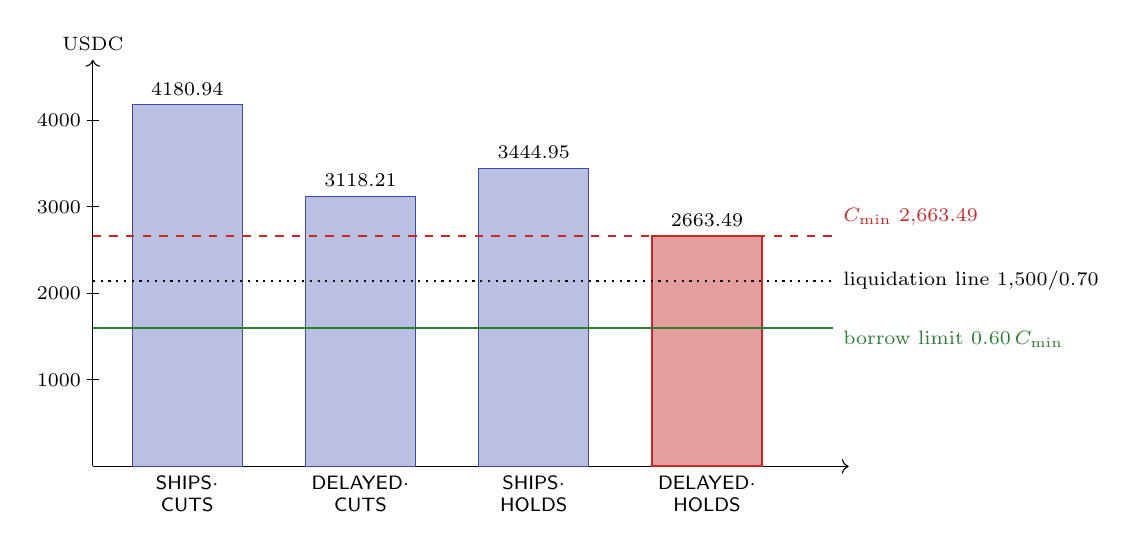
\begin{tikzpicture}[font=\small,x=1cm,y=0.0011cm]
  % axes
  \draw[->] (0,0) -- (9.6,0);
  \draw[->] (0,0) -- (0,4700) node[above,font=\scriptsize]{USDC};
  \foreach \v in {1000,2000,3000,4000} { \draw (-0.08,\v) -- (0.08,\v) node[left=3pt,font=\scriptsize]{\v}; }
  % bars
  \foreach \i/\x/\v/\la/\lb in {0/1.2/4180.94/SHIPS/CUTS,1/3.4/3118.21/DELAYED/CUTS,2/5.6/3444.95/SHIPS/HOLDS,3/7.8/2663.49/DELAYED/HOLDS}{
    \fill[ifv!35] (\x-0.7,0) rectangle (\x+0.7,\v);
    \draw[ifv] (\x-0.7,0) rectangle (\x+0.7,\v);
    \node[above,font=\scriptsize] at (\x,\v) {\v};
    \node[below,font=\scriptsize,align=center] at (\x,0) {\textsf{\la}$\cdot$\\\textsf{\lb}};
  }
  \fill[bad!45] (7.1,0) rectangle (8.5,2663.49); \draw[bad,thick] (7.1,0) rectangle (8.5,2663.49);
  \draw[dashed,thick,bad] (0,2663.49) -- (9.4,2663.49) node[right,font=\scriptsize,align=left,yshift=7pt]{$C_{\min}$ 2,663.49};
  \draw[thick,good] (0,1598.09) -- (9.4,1598.09) node[right,font=\scriptsize,align=left,yshift=-4pt]{borrow limit $0.60\,C_{\min}$};
  \draw[thick,dotted] (0,2142.86) -- (9.4,2142.86) node[right,font=\scriptsize,align=left]{liquidation line $1{,}500/0.70$};
\end{tikzpicture}
\caption{Worst-world valuation of 1,000 wNEAR posted as collateral in market 1 (Normal tier), at the world prices of
14 Nov 2026. The loan is sized by the lowest bar (\wDH). With 1,500 USDC borrowed, liquidation starts only if that
bar falls below the dotted line.}
\label{fig:worst}
\end{figure}

\subsection{Interest}

Each tier is its own pool of lenders' USDC with its own interest curve. The \textbf{utilization} is
$u = \text{borrowed} / \text{supplied}$ (capped at 1). The borrow rate per second follows a ``kinked'' line:
\begin{equation}
  r(u) =
  \begin{cases}
    r_0 + s_1 \dfrac{u}{k}, & u \le k,\\[2mm]
    r_0 + s_1 + s_2 \dfrac{u - k}{1 - k}, & u > k,
  \end{cases}
  \label{eq:rate}
\end{equation}
with base $r_0$, slopes $s_1, s_2$ and kink $k$ from Table~\ref{tab:tiers}. Interest over an interval of $\Delta t$
seconds is $B \cdot r \cdot \Delta t$ on the borrowed amount $B$, and it compounds every time the market is touched.
A share $\rho_f = 10\%$ of all interest (the \textbf{reserve factor}) goes to the tier's insurance reserve; lenders
receive the rest, so the supply rate is
\begin{equation}
  r_{\text{supply}} = r(u)\,(1-\rho_f)\,u .
  \label{eq:supply}
\end{equation}
\inwords{When few people borrow, money is cheap. As the pool fills up, the rate rises slowly; past 80\% it rises
steeply, which pulls in new lenders and pushes borrowers to repay. Borrowing stops at 90\% utilization so lenders can
always withdraw some cash.}
Live example: at 16:39 UTC on 14 November 2026 the Safe tier of market 1 had 105,050 USDC supplied and 1,330.56 USDC borrowed, a
utilization of 1.27\%. Equation~\eqref{eq:rate} gives $1\% + 4\% \times 0.0127/0.80 \approx 1.063\%$ a year, which is
exactly the 337,179,725 per second the contract reported.

Lender shares use virtual offsets ($10^6$ shares and 1 unit of assets) so the first depositor cannot inflate the
share price and steal from later depositors.

\subsection{Liquidation}

When $\mathrm{HF} < 1$ anyone can liquidate, unless the market is halted by an open outcome proposal (resolution can
only raise health factors, so liquidating during the dispute window would front-run it) or a world has no price. The
liquidator repays $r$ USDC, at most
\begin{equation}
  r_{\max} = \begin{cases}
    \text{debt}, & \mathrm{HF} < 0.90 \text{ or debt} < 200 \text{ USDC},\\
    0.5\cdot\text{debt}, & \text{otherwise},
  \end{cases}
  \label{eq:rmax}
\end{equation}
and receives the \emph{same fraction} $f$ of every collateral piece:
\begin{equation}
  \text{target} = r\,(1+b), \qquad f = \min\!\left(1,\; \frac{\text{target}}{C_{\min}}\right).
  \label{eq:seize}
\end{equation}
\inwords{The liquidator pays back part of the loan and gets that value plus a bonus (5\%, 6\% or 8\%) in collateral.
Taking the same slice of every piece keeps the borrower's worst world the worst one, so the slice is worth at least
the target in \emph{every} world. The liquidator is paid whatever happens.}
A repayment may not leave a remainder between zero and the 100 USDC minimum loan, so no dust loans are left behind.

\paragraph{Tokens or cash.} A liquidator can take the slice as tokens, or ask for \textbf{cash}: in the same
transaction the contract turns the pieces into single-world tokens, sells each world's wNEAR in its world pool, merges
the USDC-if-$w$ back into real USDC as far as every world allows, and pays it out. The liquidator sets a minimum
amount of cash; the sale also may not leave any world without a liquidation price. If either check fails, the whole
transaction is reverted.

\subsection{Insurance and bad debt}

If a liquidation takes every piece and some debt is still left, that remainder is \textbf{bad debt}. It is written off
in this order:
\begin{equation}
  \text{cover} = \min(\text{bad},\ \text{insurance}), \qquad \text{loss to lenders} = \text{bad} - \text{cover}.
  \label{eq:baddebt}
\end{equation}
\inwords{The tier's insurance reserve pays first. Only what it cannot cover is shared by the lenders of that tier, all
at once, through a lower share price.}
The insurance reserve grows from the reserve factor and from anyone who adds USDC to it with \code{fund\_insurance}.
It is never lent out. On the live contract the Bold tier of market 1 holds about 1,500 USDC of insurance. If a
market's lenders are wiped out, the market freezes.

%=====================================================================
\section{Market creation by proposals and pledges}
\label{sec:catalog}

Markets do not have to be created by the team. Anyone can propose one, and the community funds its starting
liquidity with \textbf{pledges}. A pledge is wNEAR or USDC held in escrow for a proposal: it becomes the new market's
pool liquidity when the market opens, and it is returned if the proposal ends without opening.

\subsection{Two kinds of proposal}

\begin{itemize}
  \item \textbf{Kind A} (\code{propose\_event}): a brand-new yes/no event with its question, rule, source, deadline,
  starting odds and a price multiplier per outcome (each multiplier between 0.5 and 2). The owner must approve the
  event; a market on it then opens when pledges reach the goal.
  \item \textbf{Kind B} (\code{propose\_market}): a market on one to three events that already exist and are still
  open. No approval is needed: the market \emph{opens by itself} the moment pledges reach the goal.
\end{itemize}

\subsection{Pricing a new market}

A new market needs starting prices. Origami Verse never takes them from a proposer's guess alone:
\begin{enumerate}
\item \textbf{Spot reference} $S_{\text{ref}}$. Read from the TWAP of one or more anchor markets (market 1 on the live
contract). Anchors must agree within 3\%. Because \code{require\_external} is on, $S_{\text{ref}}$ must also be within
10\% of an outside NEAR/USD reference at most an hour old.
\item \textbf{Shape.} For Kind A, the proposer's odds $q_0, q_1$ and multipliers $m_0, m_1$, normalised so that
$q_0 m_0 + q_1 m_1 = 1$. For Kind B, each event's odds and price ratios are read from its \emph{reference market}
(which must have at least 10,000 USDC of depth and agree with $S_{\text{ref}}$ within 10\%); the odds are clamped to
$[1\%, 99\%]$ and combined:
\begin{equation}
  q_w = \prod_{k} c_k\big(o_k(w)\big), \qquad m_w = \prod_k R_k\big(o_k(w)\big),
  \label{eq:kindb}
\end{equation}
where $c_k(o)$ is the clamped chance of outcome $o$ of event $k$ and $R_k(o)$ the ratio of that outcome's price to
its reference level.
\item \textbf{World prices.}
\begin{equation}
  p_w = S_{\text{ref}} \cdot \frac{m_w}{\sum_v q_v m_v},
  \label{eq:shape}
\end{equation}
so that the new market's implied spot~\eqref{eq:implied} equals $S_{\text{ref}}$. For Kind B every world price
must lie between 0.2 and 5 times $S_{\text{ref}}$.
\end{enumerate}
\inwords{A new market starts at today's real NEAR price, spread across its worlds in the proportions that existing
markets (or, for a brand-new event, the proposer's stated view within limits) already show. A proposer cannot open a
market at silly prices.}

\subsection{The goal}

The \textbf{goal} is the value of pledges needed to give every world pool a minimum depth. The planner computes the
wNEAR $A^\ast$ and USDC $U^\ast$ needed for every world pool to hold 15,000 USDC of depth (odds pools get 25\% of that
depth), then
\begin{equation}
  \text{goal} = \max\!\Big(10{,}000,\; \big\lceil A^\ast S_{\text{ref}} + U^\ast \big\rceil_{1{,}000}\Big) \text{ USDC},
  \label{eq:goal}
\end{equation}
where $\lceil\cdot\rceil_{1{,}000}$ rounds up to a multiple of 1,000. Live goals on testnet range from 39,000 USDC
(a two-world market) to 66,000 USDC (the eight-world market on three events). Pledges count at their value; a single
pledge must be at least 10 USDC or 3 wNEAR.

\subsection{Opening, refunds and the seed vault}

When the pledged value reaches the goal, the market opens in one transaction: it creates the event (Kind A), the
market, every world pool and odds pool at the planned prices, and a \textbf{seed vault} that holds the pools on
behalf of the pledgers. Each pledger receives vault shares in proportion to what the opening used of their pledge,
and gets back what it did not use. Vault shares unlock 7 days after opening. If the pledge that reaches the goal
carries enough gas, it schedules the opening itself (\code{auto\_open}); anyone can also call \code{open\_market}.
Before a market opens, a pledger can withdraw at any time.

\subsection{Bonds, reserves and spam limits}

A proposer attaches NEAR: a \textbf{bond} (0.2 NEAR for Kind A, 0.05 NEAR for Kind B) and an \textbf{opening reserve}
(0.05 NEAR plus 0.025 NEAR per world: 0.10, 0.15 or 0.25 NEAR) that pays for the new market's storage. The Kind A
bond comes back when the owner approves the event; if the owner rejects it, the owner may keep the bond for the
protocol's storage fund. A combination's bond goes to the storage fund if its proposer withdraws it. The reserve
comes back to the proposer, minus whatever an opening spends.

\begin{table}[t]
\centering
\small
\begin{tabularx}{\linewidth}{@{}Xr@{}}
\toprule
\textbf{Parameter (live value, \code{market\_params})} & \textbf{Value} \\
\midrule
Bond, Kind A / Kind B & 0.2 / 0.05 NEAR \\
Opening reserve for 2 / 4 / 8 worlds & 0.10 / 0.15 / 0.25 NEAR \\
Proposal lifetime while pledging & 60 days \\
Owner review window (Kind A) & 14 days \\
Minimum pledge window before a new event's deadline & 1 day \\
Minimum market life after opening & 3 days \\
Notice before opening after the owner changes terms & 1 hour \\
Seed vault lock after opening & 7 days \\
Depth target per world pool / minimum opening depth & 15,000 / 10,000 USDC \\
Minimum goal, goal rounding & 10,000 / 1,000 USDC \\
Odds pool depth relative to world pools & 25\% \\
Odds clamp & 1\% \\
Anchor agreement / reference agreement / outside agreement & 3\% / 10\% / 10\% \\
Minimum pledge & 10 USDC or 3 wNEAR \\
Live proposals per account / pledges per account / live proposals per event & 4 / 32 / 16 \\
Spam floor (evictable after 3 days if pledges are below this share of the goal) & 10\% \\
\bottomrule
\end{tabularx}
\caption{Market-creation parameters on the live contract.}
\label{tab:catalog}
\end{table}

To stop spam, each account may have at most 4 live proposals and each event at most 16. A proposal that is at least 3
days old and has pledges below 10\% of its goal (the \textbf{spam floor}) can be evicted to make room for a new one.

\begin{figure}[t]
\centering
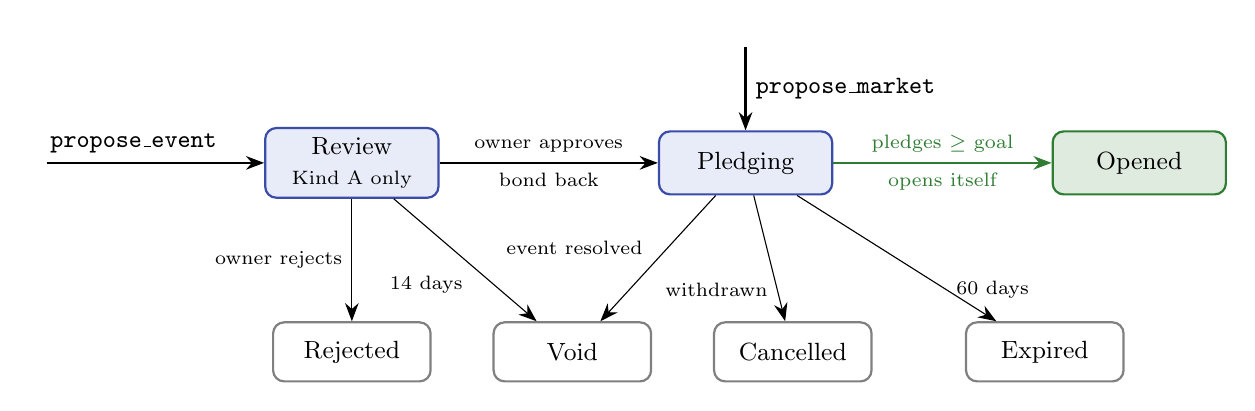
\begin{tikzpicture}[
  font=\small,
  st/.style={draw=ifv,thick,rounded corners,fill=ifvlight,minimum width=2.2cm,minimum height=0.8cm,align=center},
  end/.style={draw=gray,thick,rounded corners,fill=white,minimum width=2.0cm,minimum height=0.75cm,align=center},
  >={Stealth[length=2.3mm]}]
  \node[st] (review) at (0,0) {Review\\\scriptsize Kind A only};
  \node[st] (pledging) at (5,0) {Pledging};
  \node[st,fill=good!15,draw=good] (opened) at (10,0) {Opened};
  \node[end] (rejected) at (0,-2.4) {Rejected};
  \node[end] (void) at (2.8,-2.4) {Void};
  \node[end] (cancelled) at (5.6,-2.4) {Cancelled};
  \node[end] (expired) at (8.8,-2.4) {Expired};
  \node (startA) at (-4.0,0) {};
  \node (startB) at (5,1.6) {};
  \draw[->,thick] (startA) -- node[above,font=\scriptsize,pos=0.4]{\code{propose\_event}} (review.west);
  \draw[->,thick] (startB) -- node[right,font=\scriptsize]{\code{propose\_market}} (pledging);
  \draw[->,thick] (review) -- node[above,font=\scriptsize]{owner approves}node[below,font=\scriptsize]{bond back} (pledging);
  \draw[->,thick,good] (pledging) -- node[above,font=\scriptsize]{pledges $\ge$ goal}node[below,font=\scriptsize]{opens itself} (opened);
  \draw[->] (review) -- node[left,font=\scriptsize]{owner rejects} (rejected);
  \draw[->] (review) -- node[below left,font=\scriptsize,pos=0.55]{14 days} (void);
  \draw[->] (pledging) -- node[above left,font=\scriptsize,pos=0.55]{event resolved} (void);
  \draw[->] (pledging) -- node[left,font=\scriptsize,pos=0.75]{withdrawn} (cancelled);
  \draw[->] (pledging) -- node[right,font=\scriptsize,pos=0.75]{60 days} (expired);
\end{tikzpicture}
\caption{Proposal lifecycle. Kind A starts in Review; Kind B starts in Pledging. Pledges are accepted in Review and
Pledging. The owner can also reject a new event while it is pledging, and a proposer can withdraw a proposal
nobody has pledged to in either state (simplified here). Every grey end state refunds all pledges. Status changes are applied lazily by the first call that needs
them, so no timer is required on chain.}
\label{fig:lifecycle}
\end{figure}

%=====================================================================
\section{Resolution}
\label{sec:resolution}

\subsection{From a public source to a final outcome}

An event's outcome becomes final in one of three ways:
\begin{enumerate}
\item \textbf{Reporter.} A dedicated reporter account proposes the outcome with \code{report\_outcome}, together with
up to 512 bytes of evidence, which is logged on chain. The reporter's tools sign with a NEAR \emph{function-call key}:
it can call only \code{report\_outcome} and \code{finalize} on the contract and cannot move funds.
\item \textbf{OutLayer.} Anyone can call \code{request\_resolution} and pay OutLayer's fee. OutLayer \cite{outlayer}
runs a small pinned program inside a trusted execution environment (an Intel TDX worker) and hands the answer back to
the contract through NEP-519 yield/resume \cite{nep519}. The program's download URL and its SHA-256 hash are pinned on
chain, so a different program cannot answer. A valid answer becomes an ordinary proposal; a failed run or malformed
answer is logged and dropped.
\item \textbf{Owner.} \code{admin\_resolve} finalizes at once. This is an emergency path and is trusted.
\end{enumerate}

\subsection{The dispute window}

A proposed outcome is not final straight away. It stays open for the \textbf{dispute window}: 600 seconds (10
minutes) on the live contract. While it is open, every market that uses the event is \emph{halted}: swaps in its
pools, order fills and liquidations stop, so nobody can trade on the answer before it is final. During the window
the owner may \code{dispute}, which cancels the proposal (a new one may follow). After the window, \emph{anyone} can
call \code{finalize}.

\begin{figure}[t]
\centering
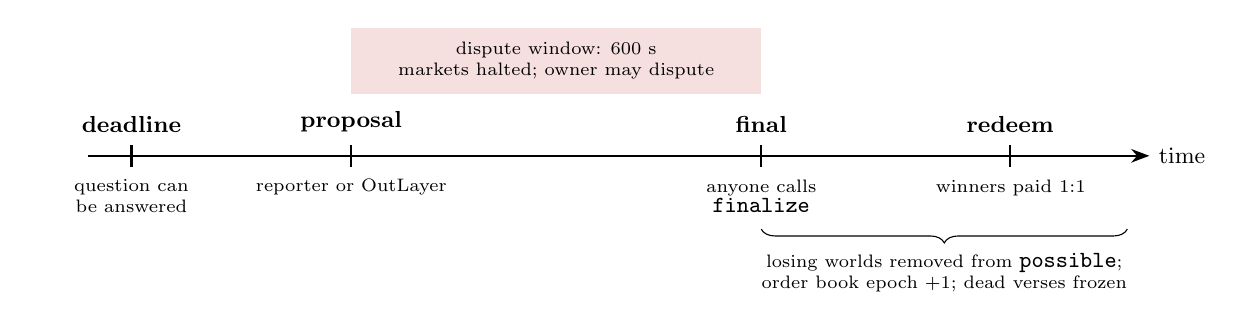
\begin{tikzpicture}[font=\small,>={Stealth[length=2.3mm]},scale=0.93,transform shape]
  \draw[->,thick] (0,0) -- (14.5,0) node[right]{time};
  \foreach \x/\lab/\sub in {0.6/deadline/question can be answered,3.6/proposal/reporter or OutLayer,9.2/final/anyone calls \code{finalize},12.6/redeem/winners paid 1:1}{
    \draw[thick] (\x,-0.15) -- (\x,0.15);
    \node[above,font=\small\bfseries] at (\x,0.2) {\lab};
    \node[below,font=\scriptsize,align=center,text width=2.6cm] at (\x,-0.2) {\sub};
  }
  \fill[bad!15] (3.6,0.85) rectangle (9.2,1.75);
  \node[font=\scriptsize,align=center] at (6.4,1.3) {dispute window: 600 s\\markets halted; owner may dispute};
  \draw[decorate,decoration={brace,amplitude=5pt,mirror}] (9.2,-1.0) -- (14.2,-1.0)
    node[midway,below=6pt,font=\scriptsize,align=center]{losing worlds removed from \code{possible};\\order book epoch $+1$; dead verses frozen};
\end{tikzpicture}
\caption{Resolution timeline of one event.}
\label{fig:timeline}
\end{figure}

\subsection{Finalize and redeem}

Finalizing an event resolves every market that uses it. Worlds whose outcome for that event differs from the final
one are removed from \code{possible}. The market's resolution count goes up, which closes every resting order of the
old epoch. Verses whose masks lost all their worlds are dead and can no longer move. Once every event of a market is
final, exactly one world is left; the verse tokens covering it are collapsed and redeem one for one into real wNEAR
or USDC. Borrowers can close their loan and redeem in a single call (\code{close\_after\_resolution}).

\subsection{Examples on testnet}

\begin{itemize}
\item Event 3, ``Did the Fed cut at its October 27--28, 2026 meeting?'', was resolved through OutLayer. The pinned
program reads the FRED series DFEDTARU and DFEDTARL \cite{fred}: the upper and lower limits were 4.00\% and 3.75\%
both before and after the meeting, so the answer is \textsf{HOLDS}. The chain shows the event final with outcome \textsf{HOLDS} and
\code{proposed\_by: "outlayer"}. On the first deployment the same program ran in 1,655 ms and OutLayer charged
0.0011655 NEAR of the 0.005 NEAR deposit, refunding the rest.
\item Event 4, ``Did NEAR close above \$4.00 on Nov 1, 2026?'', was reported by the reporter from the Coinbase daily
close (4.284 USDC, with Kraken's 4.2827 as supporting evidence) and finalized after the 10-minute window. Outcome:
\textsf{YES}.
\end{itemize}

%=====================================================================
\section{The outside NEAR/USD reference}
\label{sec:reference}

Lending prices come from Origami Verse's own pools. If those pools drift away from the real world (for example because
nobody trades them on testnet), loans could be sized on stale prices. Origami Verse therefore keeps an outside
\textbf{reference price} $R$ for NEAR/USD.

\subsection{How the reference is formed}

The reference is the \emph{median} of NEAR/USD from four public sources: Coinbase, Kraken, Gemini and CoinGecko. It
can be written by a pinned OutLayer program (\code{oracle/nearusd-guest}) or by the reporter key. Every new value,
from either path, must have been observed at most 300 seconds before it arrives and no more than 60 seconds in the
future, must be newer than the stored one, and must lie between 0.1 and 1,000 USDC. For a value from the OutLayer
program the contract also checks that at least 3 sources answered and that they agree within 2\% (200 bps). The
reporter path sends only the price and its time, so the keeper applies the same 3-source, 200 bps rule off chain
before it posts.

Example: the seed price of the live markets was the median of Coinbase 3.3204, Kraken 3.3230, CoinGecko 3.33 and
Gemini 3.3477 at 04:32 UTC on 14 November 2026. With four sources the median is the mean of the middle two:
$(3.3230 + 3.33)/2 = 3.3265$, with a spread of 83 bps.

\subsection{How lending uses it}

For each market with the check switched on, the contract compares the reference with the implied spot
of~\eqref{eq:implied} computed from TWAPs:
\begin{equation}
  \rho = \frac{R}{S_{\text{implied}}}, \qquad
  f_b = \min(\rho, 1), \qquad
  f_l = \begin{cases} 1, & \rho \ge 1,\\ \max(\rho,\; 1 - h), & \rho < 1, \end{cases}
  \label{eq:rho}
\end{equation}
with maximum haircut $h = 20\%$ on the live markets. Then:
\begin{itemize}
\item \textbf{New borrowing is blocked} if the reference is older than 3,600 seconds, or if $|\rho - 1| > 10\%$.
\item If the pools sit \emph{above} the real price ($\rho<1$), both sides are scaled down by $\rho$ (the
liquidation side by at most 20\%), using a reference at most 300 seconds old for liquidation.
\item If the pools sit more than 10\% \emph{below} the real price ($\rho > 1.1$), liquidation waits (the
\emph{guard}): it would be unfair to liquidate someone on prices the outside world does not confirm.
\item Repaying, adding collateral, withdrawing supply and exiting never wait on the reference.
\end{itemize}
\inwords{The protocol checks its own prices against real exchanges. If its pools say NEAR is worth much more than
the exchanges do, it lends less. If they disagree too much, it stops new loans until they agree again. It never
traps anyone: you can always repay and leave.}

\subsection{Limits of the check}

The reference covers \emph{today's} NEAR price only. It cannot say what NEAR \emph{would} be worth in a particular
world, so it checks the weighted average~\eqref{eq:implied}, not each world price. It depends on the odds being
right; on the live markets one set of odds is an assumption (Section~\ref{sec:trading}). On the testnet deployment the
reference is written by the reporter path; the OutLayer program for NEAR/USD is built and its hash is fixed, but it
is not yet configured on the live contract.

%=====================================================================
\section{Implementation on NEAR}
\label{sec:near}

\subsection{One contract}

On NEAR, a call to another contract is asynchronous: it runs in a later receipt, and if it fails, the caller is not
rolled back \cite{neardocs}. A hedge that splits, fills orders, swaps in several pools, posts collateral and borrows
would need a callback and a compensation path at every step if each part were a separate contract. Origami Verse puts
pools, order book, lending, proposals and the liquidity vault in \emph{one} contract, so such a hedge is one
synchronous call that either fully succeeds or fails and changes nothing. The only calls that leave the contract are
payouts of real tokens (after every state change), the NEP-245 transfer-call receiver, NEAR refunds and OutLayer
requests.

The contract is written in Rust with \code{near-sdk} 5.14 \cite{nearsdk}. The maths lives in a separate crate with no
NEAR dependency: fixed-point arithmetic with 256- and 512-bit intermediates, tick maths ported from Uniswap v4's
TickMath \cite{uniswapv4}, constant-product pools, the dynamic fee, TWAP, odds, shares, order maths, the opening
planner and worst-world risk. Rounding always favours the protocol: what a user receives rounds down, what a user
pays rounds up.

\subsection{Tokens in and out}

Real wNEAR and USDC (NEP-141 tokens \cite{nep141}) enter only through \code{ft\_transfer\_call}. Its \code{msg} field
names the action, for example \code{split}, \code{conditional\_sell}, \code{sell\_and\_borrow}, \code{post\_order},
\code{supply}, \code{repay}, \code{deposit\_collateral}, \code{liquidate}, \code{pledge} or \code{fund\_insurance}.
There is no separate approval step. The contract returns the part the action did not use, and the token contract
refunds it; if any check fails the call panics and the token contract refunds everything. Inside the contract every
amount has 18 decimals: USDC (6 decimals) converts exactly; for wNEAR (24 decimals) the part below one internal unit
is sent straight back. Payouts use \code{ft\_transfer} with a 5 Tgas callback that credits the amount back if the
transfer fails (for example when the receiver is not registered with the token).

\subsection{Storage staking}

NEAR charges for on-chain storage by locking NEAR \cite{nep145}. Origami Verse implements NEP-145: an account registers with
at least 0.1 NEAR. Every state-changing call measures storage before and after, charges the bytes it adds to the
payer's deposit (failing if the deposit does not cover them) and credits the bytes it frees. Zero balances are deleted
so they stop costing storage. A new market's storage is paid from its proposer's opening reserve, then from a
protocol storage fund. The contract code itself (1,380,136 bytes) locks about 13.8 NEAR at NEAR's price of
$10^{19}$ yoctoNEAR per byte.

\subsection{Gas}

A NEAR transaction may attach at most 300 Tgas. The web app attaches 150 Tgas to routine token calls (split, sell or
buy from the wallet, supply, repay, deposit collateral) and the full 300 Tgas to pledges, liquidations, proposals,
openings and resolution requests. World trades from the order screen attach 20 Tgas per order fill, 30 per pool swap
and 25 per posted order. A pledge schedules an automatic opening only if 215 Tgas are still left. The OutLayer
callback receives 20 Tgas. Testnet buys the attached gas up front and refunds what is not burnt, so an everyday
action needs about 0.17 NEAR free while signing but costs about 0.001 NEAR. A reference update by the keeper burnt
3.7 Tgas (0.00035 NEAR).

\subsection{Events, views and keys}

Every action logs a NEP-297 event \cite{nep297} under the standard \code{multiverse}, and every balance change logs
NEP-245 \code{mt\_mint}, \code{mt\_burn} or \code{mt\_transfer}. Views are designed one per screen, because NEAR RPC has
no batching. The reporter signs with function-call keys limited to \code{report\_outcome}, \code{finalize} and
\code{report\_reference}.

\subsection{Upgrades and pausing}

The contract carries a code version (2.0.0) and a state version (2). An upgrade deploys the new code and runs
\code{migrate} in the \emph{same} transaction, so a failed migration reverts the deployment as well. Ownership moves
in two steps (propose, then accept). The owner, or an optional guardian, can pause narrow parts of the system with
separate flags: trading, lending, minting, transfers, liquidation, the oracle, pledging and exits. After an unpause,
liquidations can be held back by a grace period of at most 86,400 seconds so borrowers have time to react.

\subsection{The keeper}

A hosted \textbf{keeper} (a serverless function next to the web app) does three jobs in each round: it posts the
NEAR/USD reference when the stored one is at least 300 seconds old; it keeps the lendable market close to the
reference by trading back towards it when the implied spot is more than 4\% away (and leaves gaps over 25\% to a
person); and it liquidates unhealthy loans, taking cash only when the cash covers the repayment after a 0.5\% margin.
It runs when anyone has the site open (at most once a minute per browser), on a daily cron and from an external
scheduler every 30 minutes. Two rounds cannot double-send: each key signs with a nonce derived from the block height
rounded down to 100 blocks, so a second round in the same window is rejected by the chain at no cost.

%=====================================================================
\section{Security and invariants}
\label{sec:security}

\subsection{What the contract checks}

\begin{itemize}
\item \textbf{Backing} (Equation~\ref{eq:backing}) for every market, asset and possible world, and that the contract's
real token balance equals reserves plus users' internal balances.
\item \textbf{Dead stays dead}: nothing on a dead verse succeeds and its supply never changes.
\item \textbf{Resolution never lowers a health factor.}
\item \textbf{Liquidation covers the repayment}: when the worst-world value covers repayment plus bonus, the seized
slice is worth at least the repayment in every possible world.
\item \textbf{Order escrow}: every open bid holds at least the cost of what remains, every open ask exactly what
remains.
\item \textbf{No fill after resolution or expiry}, and only the maker can cancel.
\end{itemize}
Each is a stateful property test: random sequences of 50 to 200 actions (256 cases each, and 24 to 40 cases on
eight-world markets), with the invariant checked after every step. Market-creation invariants (pledges, refunds, openings) have
their own randomised tests. The full Rust suite had 856 passing tests at the last recorded integration run.

\subsection{Internal review}

Before version 2, the team reviewed the first version and recorded ten findings (two high, four medium, four low),
each first reproduced by a failing test and kept as a regression test. The two high findings were about lending
prices coming from the protocol's own pools, which then used a 60-second TWAP: pumping every world pool for one
window could unlock too much borrowing, and dumping one world pool for one window could liquidate a healthy borrower.
Both are mitigated, not removed: the 30-minute TWAP, the price states of Section~\ref{sec:prices}, the
borrow/liquidation split and, in version 2, the outside reference. The version 2
specification went through an adversarial review of its economics, runtime limits, migration and completeness before
it was implemented.

\subsection{What is not covered}

\begin{itemize}
\item There has been \textbf{no external audit}. The review above was done by the people who built the system.
\item The owner is trusted: \code{admin\_resolve} finalizes at once and only the owner can dispute. There is no
timelock and no multisig.
\item One reporter key proposes outcomes and posts the reference. If the owner does not dispute a wrong proposal in
time, anyone can finalize it.
\item Someone who holds a pool at a false price for a whole TWAP window still moves it; on testnet few people
arbitrage it back. The outside reference limits but does not remove this.
\item wNEAR and USDC on testnet are mock tokens with an open mint; they have no value.
\end{itemize}

%=====================================================================
\section{Deployment and evaluation on testnet}
\label{sec:eval}

\subsection{Accounts}

Origami Verse v2 runs on NEAR testnet. The contract is \code{app.ifverse-staging.testnet} (code hash
\code{9K62NFX7gQiGajRuLTFcPy7F9n5nADSrFgESttUSFcRR}, deployed in transaction
\tx{C3KthRtFPyJa68XRXNqBjvE6LpTqZfPgKsAo2U73bcpU}{C3KthRtFPy}). Mock wNEAR (24 decimals) and USDC (6 decimals) live at
\code{wnear.ifverse-staging.testnet} and \code{usdc.ifverse-staging.testnet}. The reporter, keeper and maker have their own sub-accounts. The
web app is at \url{https://multiverse-lending.vercel.app}. Transaction hashes below are shortened; each is a link
to its full record on \url{https://testnet.nearblocks.io}.

\subsection{Live markets}

\begin{table}[t]
\centering
\small
\begin{tabularx}{\linewidth}{@{}c>{\raggedright\arraybackslash}Xcllr@{}}
\toprule
\textbf{Id} & \textbf{Events} & \textbf{Worlds} & \textbf{Origin} & \textbf{Status} & \textbf{Goal} \\
\midrule
1 & SPICE $\times$ Fed December (lending, three tiers) & 4 & team (anchor) & open & -- \\
2 & Fed October (past) & 2 & team & resolved \textsf{HOLDS} & -- \\
3 & NEAR close $>$ \$4.00 on Nov 1 (past) & 2 & team & resolved \textsf{YES} & -- \\
4 & Fed December & 2 & Kind B, proposal 1 & open & 42,000 \\
5 & SPICE & 2 & Kind B, proposal 2 & open & 41,000 \\
6 & NEAR close $>$ \$3.25 on Dec 31 & 2 & Kind A, proposal 3 & open & 40,000 \\
7 & SPICE $\times$ NEAR Dec 31 & 4 & Kind B, proposal 4 & open & 54,000 \\
8 & SPICE $\times$ Fed Dec $\times$ NEAR Dec 31 & 8 & Kind B, proposal 5 & open & 66,000 \\
9 & NEAR mainnet $>$ 30M txs in Dec 2026 & 2 & Kind A, proposal 14 & open & 39,000 \\
10 & Fed December $\times$ NEAR Dec 31 & 4 & Kind B, proposal 15 & open & 55,000 \\
\bottomrule
\end{tabularx}
\caption{Markets on \code{app.ifverse-staging.testnet} (\code{list\_markets}, 14 Nov 2026). Goals are in USDC. Seven of
the ten markets were opened by proposals and pledges, not by the team. By 16:40 UTC on 14 November, 21 proposals
had been made.}
\label{tab:markets}
\end{table}

Table~\ref{tab:markets} lists the ten markets. Market 1 is the lending market: each of its tiers was supplied with
about 100,000 USDC, and at 16:39 UTC on 14 November 2026 each tier had two borrowers (Safe 1,330.56, Normal 2,641.09 and Bold
2,504.25 USDC borrowed). Pledged markets have world pools of roughly 15,000--20,000 USDC each, below the 50,000 USDC
depth lending requires, so they are trading-only until they deepen.

\subsection{Real transactions}

All flows were exercised with real testnet transactions. A selection:
\begin{itemize}
\item Split, sell and buy on market 1: \tx{DadzKfXqrV613gPLeWdWn2CHNC196fueGW1GZJpTguj2}{DadzKfXqrV},
\tx{FJf2F6YKWUQuQmxjAcoHbkx3b9dZEpeY4MSxfVVvWJvz}{FJf2F6YKWU}, \tx{C5hCvxEWDFefWbcg6kmdgBqzuE2xBuXDVuvbZ27LUg7k}{C5hCvxEWDF}.
\item A four-world hedge in one call (sell in three worlds, keep the fourth):
\tx{8tBtiLdLGcA8UFwQRQ3Aiy5AbvYrujHuMHBQ2ZLqqQZD}{8tBtiLdLGc}.
\item Order place, cancel and fill: \tx{8vCsyVaizg5bTDT2y5bP1ttAeHK8YSfZMQtT2oBRJdF1}{8vCsyVaizg},
\tx{2WaRDhGcT3yvhdDfbbgWxrBD9EG7KNbHiRbVwrwmBcSW}{2WaRDhGcT3}, \tx{BoDLFFgRqFwYKV9cFMPaQ9krsqWnw9qp2bJowyP1zQN3}{BoDLFFgRqF}.
\item Borrow in the Bold tier: \tx{F41xJKvnvHndEC5EYAH2N5NXm3PwF8LL6Cf7mSrGWtpA}{F41xJKvnvH}.
\item A Kind A proposal and its approval, then a Kind B proposal and the pledge that opened its market:
\tx{39Eu1oWYGZHmj9pMJRsJhVuNenVjzeRLp1QUFXWfZVnz}{39Eu1oWYGZ}, \tx{7etK5dUxeD6hRCi2n9j1RhLDunZ9PUcKdx6xrdeSYkGp}{7etK5dUxeD},
\tx{F69pf735E5XLuRnzUJ8hggD5S6bG7AtMQ5b228qXPwZX}{F69pf735E5}, \tx{5vFZLCzAniB96gvVsudAY9WuMcKqk42ddxh8NXqAViAR}{5vFZLCzAni}.
\item A Kind A proposal recorded for the walkthrough video (it became market 9): \tx{91RJbDnwkxqhUjUYAyiA6Nz9LfgL9P4BcHwNjTSgwru}{91RJbDnwkx}.
\item Reference update by the keeper: \tx{HTYgfTkHfxvfAxxE5mGNQn5cNcJXAUashCB7b8Xk9cCc}{HTYgfTkHfx} (3.33245, from four sources
with a 114 bps spread).
\end{itemize}

\subsection{A real liquidation}

To show liquidation end to end, one account sold 17,600 wNEAR-if-\wDH{} into that world's pool, moving NEAR's price
in \wDH{} from about 2.61 to 1.58 USDC. As the 30-minute average followed, a Bold-tier borrower's health factor fell
from 1.21 to 0.98 in about 12 minutes. One keeper round found the loan and liquidated it
(\tx{4p5K22NqtujzJQXn9Gnxsrpa5s1KJG5Xh2NwEiJkwYVh}{4p5K22Nqtu}). It chose tokens rather than cash, because selling the seized
wNEAR into the pushed pool would not have covered the repayment, exactly the rule the keeper follows. The price was
then bought back.

\subsection{Keeper behaviour}

In testing, two keeper rounds raced in the same 100-block window: one landed
(\tx{FPmqoG6kh4mcRr8gn3b5xZ7ixQK4HreTRKuYSDw63XPt}{FPmqoG6kh4}) and the other was rejected for its nonce without reaching
the chain, as designed. In two later recorded rounds the market maker step found market 1 within its 4\% band
(42 and 10 basis points from the reference), so it sent nothing, and borrowing stayed open.

%=====================================================================
\section{Limitations and future work}
\label{sec:limits}

\begin{itemize}
\item \textbf{Testnet only.} Nothing has been deployed or tested on mainnet. Tokens are mock tokens.
\item \textbf{Trusted roles.} The owner can resolve and dispute; one reporter proposes outcomes and posts the
reference. Future work: a timelock, a multisig owner, bonded reporters and open disputes.
\item \textbf{Liquidity.} Lending reads only Origami Verse's own pools. On testnet they are deep only where the team and
pledgers put liquidity, and few people arbitrage them. Only market 1 is lendable today.
\item \textbf{Odds sources.} The SPICE odds are an assumption and the Fed odds a dated reading; a live outside odds
feed would make implied prices more meaningful.
\item \textbf{Slow price response.} Because lending uses a 30-minute average, a real price move reaches borrowing
limits and liquidations over up to 30 minutes.
\item \textbf{Events.} A market combines at most three binary events (eight worlds). Events with more than two outcomes
are not supported.
\item \textbf{Reference path.} The NEAR/USD reference is written by the reporter on testnet; the pinned TEE program for
it is built but not yet configured on the live contract.
\item \textbf{Audit.} An external security audit is required before any real value is involved.
\end{itemize}

%=====================================================================
\section{Conclusion}

Origami Verse turns ``what if'' into something you can hold. A real asset splits into one token per possible world, each
world gets its own price, and a loan is judged by the worst world that can still happen, so it stays covered whatever
the news. Around this core sit dynamic-fee pools, an order book, three lending tiers with insurance, markets that
anyone can propose and fund, resolution from public data with a dispute window and a TEE option, and an outside
price check. The whole system is one NEAR contract, live on testnet, with every number in this paper readable from
its code and views.

%=====================================================================
\begin{thebibliography}{99}
\footnotesize\raggedright
\setlength{\itemsep}{0pt}
\bibitem{white2025} D.~White. \emph{Multiverse Finance}. Paradigm, May 2025.
\url{https://www.paradigm.xyz/2025/05/multiverse-finance}

\bibitem{neardocs} NEAR Protocol documentation. \url{https://docs.near.org}

\bibitem{nearsdk} near-sdk-rs, the Rust SDK for NEAR smart contracts. \url{https://github.com/near/near-sdk-rs}

\bibitem{nep141} NEP-141: Fungible Token Standard. \url{https://github.com/near/NEPs/blob/master/neps/nep-0141.md}

\bibitem{nep145} NEP-145: Storage Management. \url{https://github.com/near/NEPs/blob/master/neps/nep-0145.md}

\bibitem{nep245} NEP-245: Multi Token Standard. \url{https://github.com/near/NEPs/blob/master/neps/nep-0245.md}

\bibitem{nep297} NEP-297: Events. \url{https://github.com/near/NEPs/blob/master/neps/nep-0297.md}

\bibitem{nep519} NEP-519: Yield Execution. \url{https://github.com/near/NEPs/blob/master/neps/nep-0519.md}

\bibitem{outlayer} OutLayer: verifiable off-chain execution for NEAR (contract \code{outlayer.testnet}).
\url{https://app.outlayer.ai}

\bibitem{uniswapv3} H.~Adams, N.~Zinsmeister, M.~Salem, R.~Keefer, D.~Robinson. \emph{Uniswap v3 Core}. 2021.
\url{https://uniswap.org/whitepaper-v3.pdf}

\bibitem{uniswapv4} Uniswap v4 core, \code{TickMath}. \url{https://github.com/Uniswap/v4-core}

\bibitem{fred} Federal Reserve Bank of St.\ Louis, FRED series DFEDTARU and DFEDTARL.
\url{https://fred.stlouisfed.org/series/DFEDTARU}

\end{thebibliography}

\end{document}
